\documentclass[11pt,aspectratio=1610,dvipsnames]{beamer}
\graphicspath{{figs/}}
\usetheme{default}
\usepackage{DasBeamerPaket}
\usepackage{animate}
\usepackage{lastpage}
\usepackage{tikz}
\usepackage{braket}
\usepackage{lmodern}

\usepackage{draftwatermark}
\setbeamercolor{background canvas}{bg=}%transparent canvas

\setbeamercolor{section in toc}{fg=NavyBlue}
\setbeamercolor{frametitle}{fg=NavyBlue}
\captionsetup[figure]{labelfont=bf}
\captionsetup[table]{labelfont=bf}
\setbeamertemplate{caption}[numbered]
\title[$\Lambda(1405)$]{Experimental studies of the $\Lambda(1405)$}
\subtitle[Seminar physics654]{physics654 -- Seminar on exotic multi-quark states}
\graphicspath{{figs/}}
\begin{document}
\definecolor{myWhite}{rgb}{1,1,1}

\setbeamertemplate{footline}[text line]{\parbox{0.3\linewidth}{\vspace*{-9pt}\textcolor{white} \insertsection  \hfill} \parbox{0.7\linewidth}{\vspace*{-8pt} \textcolor{white}{\hfill\hspace{-3cm}\insertshorttitle \phantom{ }-- \insertshortsubtitle}  \hfill \textcolor{myWhite}{\insertframenumber/\inserttotalframenumber}}}

\addtobeamertemplate{footline}{ \makebox[0pt][l]{\hspace{-1cm}
		\raisebox{0cm}[0pt][0pt]{\colorbox{gray!20!black}{\phantom{{\large TEXTTEXTTEXTTEXTTEXTTEXTTEXTTEXTTEXTTEXTTEXTTEXTTEXTTEXTTEXTTEXTTEXTTEXTTEXTTEXTTEXTTEXTTEXTTEXTTEXTTEXTTEXTTEXTTEXTTEXTTEXTTEXTTEXTTEXTTEXTTEXTTEXTTEXTTEXTTEXT}}}}}}

\setbeamercovered{transparent}
\setbeamertemplate{navigation symbols}{}
\setbeamertemplate{frametitle}[default][left,leftskip=0.5cm]
%
\setbeamertemplate{itemize item}{\color{black}$\blacktriangleright$}
\setbeamertemplate{section in toc}[sections numbered]
\captionsetup{font=scriptsize,labelfont=scriptsize}

\AtBeginSection[]
{	
	\definecolor{myWhite}{rgb}{0,0,0}
	\begin{frame}[noframenumbering]
		\frametitle{}
		\addtocounter{page}{-1}
		\tableofcontents[currentsection]
		
	\end{frame}
\definecolor{myWhite}{rgb}{1,1,1}
}


\begin{frame}[plain]
	\setcounter{page}{0}
	\centering
	{\Large \color{MidnightBlue}{Experimental studies of the $\Lambda(1405)$}}\\
	{\href{https://www.youtube.com/watch?v=oHg5SJYRHA0}{physics654 -- Seminar on exotic multi-quark states}}
	

	\vfill

		



			
	\textsc{Jakob Krause}\\
	\scriptsize \href{mailto:krause@hiskp.uni-bonn.de}{\faEnvelope  \hspace*{0.1cm}krause@hiskp.uni-bonn.de} {\color{black}$|$} \href{https://github.com/krausejm}{\faGithub  \hspace*{0.1cm}krausejm}\\
	
	\vspace{.5cm}
	
	Tutor: \textsc{Georg Scheluchin}\\
	 \href{mailto:scheluchin@physik.uni-bonn.de}{\faEnvelope  \hspace*{0.1cm}scheluchin@physik.uni-bonn.de}

	\vspace{0.2cm}
	
	18.06.2021
	 	
 		
\end{frame}
\section*{Motivation}
\begin{frame}{Motivation}
\begin{minipage}{\linewidth}
		\begin{tcolorbox}[colback=black!10,colframe=gray!20!black,title=What is special about the $\Lambda(1405)$?] 
			\begin{itemize}
				\item mass does not fit well into constituent quark models 
				\item invariant mass distribution (line shape) differs significantly from usual \textsc{Breit-Wigner} shape
				\item candidate for an exotic multiquark state (bound system of $\overline{K}N$) since its mass lies just below production threshold
			
 			\end{itemize}
 		\vspace{.5cm}
 		there are  many different theoretical approaches to explain this behavior\\
 		$\to$ need for more experimental data!
		\end{tcolorbox}

\end{minipage}




	
\end{frame}
%\begin{frame}[plain]
%	\maketitle
%	\setcounter{page}{0}
%\end{frame}
\section*{Table of contents}
\begin{frame}{Table of contents}
	\tableofcontents
\end{frame}
\section{Experimental setup}
\begin{frame}{Continuous Electron Beam Accelerator Facility (CEBAF)}
	\begin{figure}
		\centering
		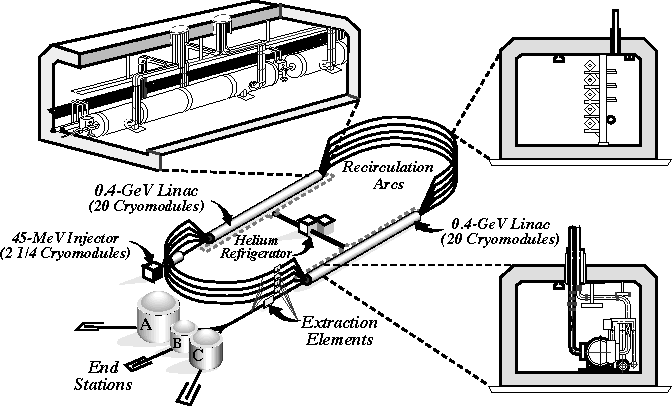
\includegraphics[width=.8\linewidth]{cebaf}
		\caption*{CEBAF layout at Jefferson Lab, [\cite{clas}]}
	\end{figure}
\end{frame}


\begin{frame}{Continuous Electron Beam Accelerator Facility (CEBAF)}
	\begin{figure}
			\centering
			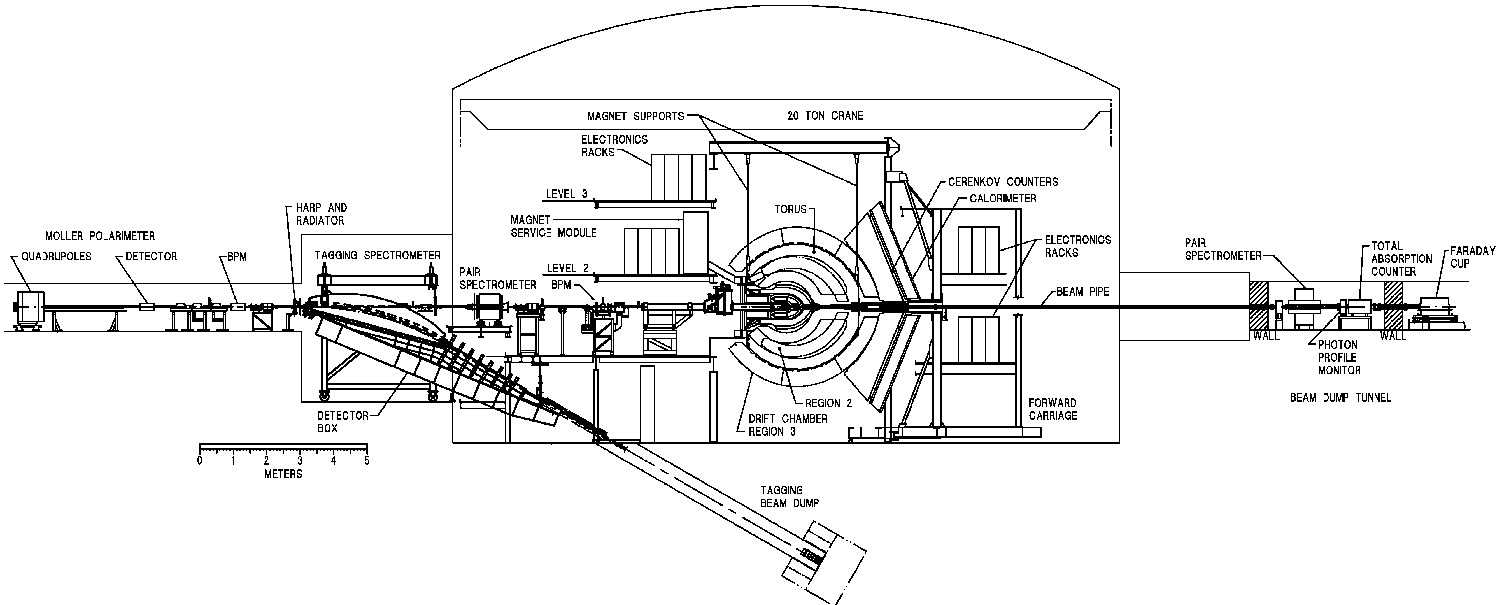
\includegraphics[width=\linewidth]{figs/tagger.png}
			\caption{Overview of the CLAS detector setup, including the tagger, \citet{clas}}
	\end{figure}
\end{frame}


\begin{frame}{CEBAF Large Acceptance Spectrometer (CLAS)}
	\begin{figure}
		\centering
		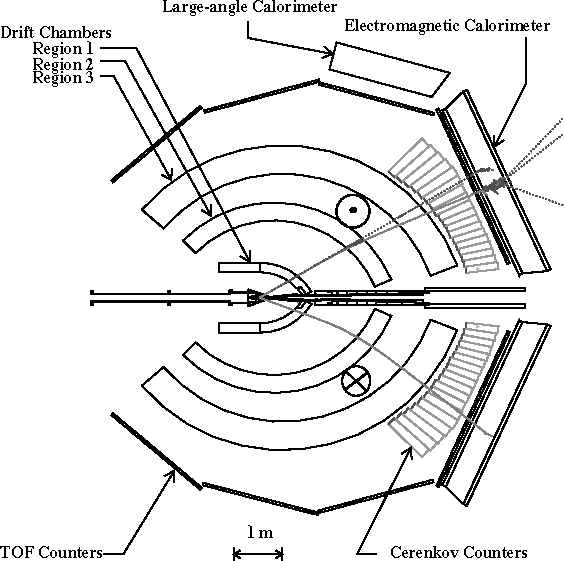
\includegraphics[width=.5\linewidth]{clas}
		\caption*{CLAS layout at Jefferson Lab, [\cite{clas}]}
	\end{figure}
\end{frame}


\section{Line-shape measurement}


\begin{frame}{Reaction kinematics}
	\begin{minipage}{.63\linewidth}
		\begin{figure}[H]
			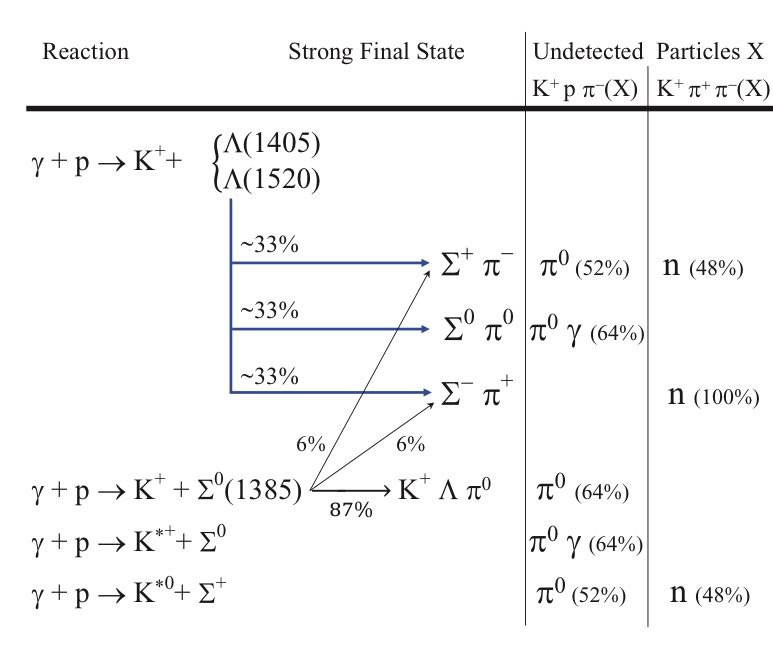
\includegraphics[width=\linewidth]{kinematics}
			\caption*{Possible and studied reactions in the analysis of the lineshapes of $\Lambda(1405)$,  \citet{lineshapes}}
		\end{figure}	
	\end{minipage}
	\begin{minipage}{.34\linewidth}
		\begin{align*}
			\Sigma^+\to &p \pi^0\\
			\Sigma^+\to &n \pi^+\\
			\Sigma^0\to &\gamma\Lambda&\to\gamma p \pi^-\\
			\Sigma^-\to &n \pi^-\\
			\Lambda\to &p \pi^-\\
		\end{align*}
	\end{minipage}
	
\end{frame}

\begin{frame}{Event selection}
two sets of reactions that the detector sees
	
	\begin{enumerate}
		\item $K^+p\pi^-(X)$
		\item $K^+\pi^+\pi^-(X)$
	\end{enumerate}
there are many cuts that can be made that apply to both
	\begin{tcolorbox}[colback=black!10,colframe=gray!20!black,title=Initial selection of particles] 
		\begin{itemize}
			\item particle identification using TOF counters and momentum measurements
			\item kinematic cuts from \textsc{Monte Carlo}
			
		\end{itemize}
	\end{tcolorbox}
\end{frame}
\begin{frame}{Event selection -- Particle identification}
\begin{figure}
	\centering
	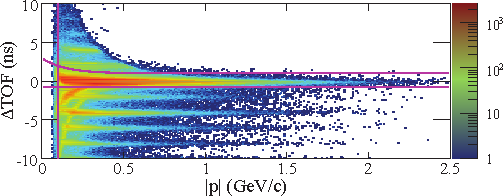
\includegraphics[width=\linewidth]{tof_pi}
	\caption*{$\Delta$TOF for $\pi^+$ @ $2.35 < W < \SI{2.45}{\giga\eV}$, applied cuts are shown in magenta. \citet{lineshapes}}
\end{figure}
\end{frame}

\begin{frame}{Event selection}
	\begin{tcolorbox}[colback=black!10,colframe=gray!20!black,title=Binning of data] 
	the data was divided:
	\begin{itemize}
		\item 10 bins in $W=\sqrt{s}$ dividing \SIrange{2}{3}{\giga\eV} in steps of \SI{100}{\mega\eV}
		\item 20 bins in $\cos\theta_\text{CMS}^{K^+}$ dividing $-1$ to $1$ in steps of $0.1$
	\end{itemize}
\end{tcolorbox}
$\to$ the following analysis was performed independently in every bin of energy and angle!
\end{frame}
\begin{frame}{Event selection}
	\centering
	\begin{minipage}{.49\linewidth}
		\begin{tcolorbox}[colback=black!10,colframe=gray!20!black,title=extracting $\Lambda\pi^0$ and $\Sigma^+\pi^-$] 
		- reminder: $\Lambda\to p\pi^-, \Sigma^+\to p\pi^0$\\	
		- final state particles: $K^+p\pi^-(\pi^0)$ 
		- determine $p_\pi$ via missing mass fit\\
		- apply cuts based on fits to the invariant masses $M_{p\pi^-}$ and $M_{p\pi^0}$	
			
			
	\end{tcolorbox}	
\end{minipage}
\begin{minipage}{.49\linewidth}
	\begin{tcolorbox}[colback=black!10,colframe=gray!20!black,title=extracting $\Sigma^+\pi^-$ and $\Sigma^-\pi^+$] 
	- reminder: $\Sigma^\pm\to n\pi^\pm$\\
	- final state particles: $K^+\pi^+\pi^-(n)$\\
	- determine $p_n$ via missing mass fit\\
	- apply cuts based on fits to the invariant masses $M_{n\pi^\pm}$
	\end{tcolorbox}	
\end{minipage}
\begin{figure}[H]
	\centering
	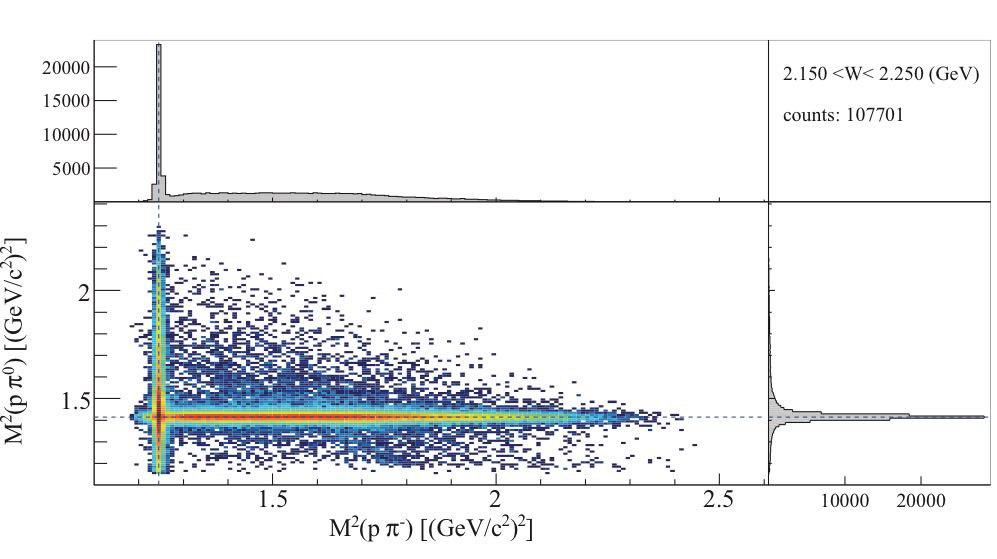
\includegraphics[width=.49\linewidth]{inv_mass_1}
	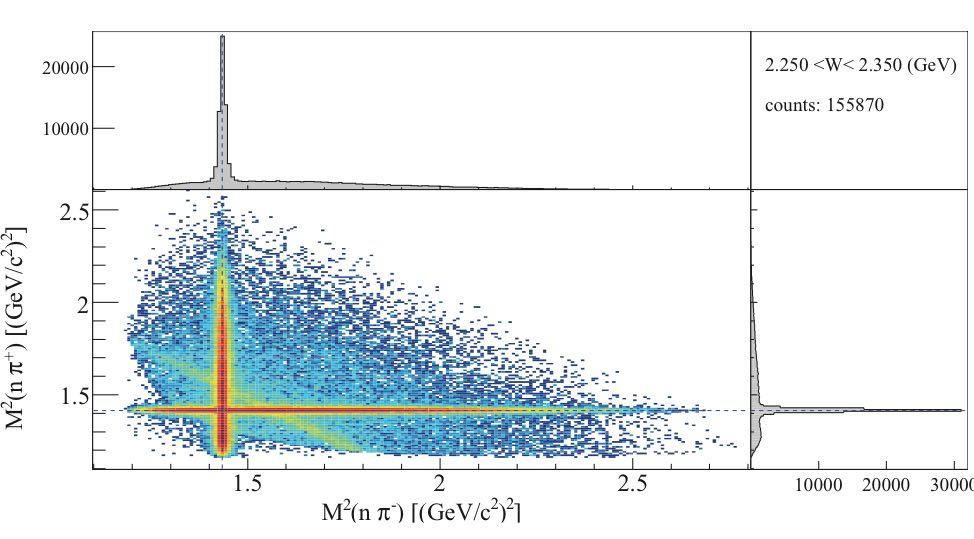
\includegraphics[width=.49\linewidth]{inv_mass_2}
	\caption*{\textsc{Dalitz}-like plots of the above mentioned invariant masses,  \citet{lineshapes}}
\end{figure}
\end{frame}

\begin{frame}{Event selection}
	\begin{minipage}{\linewidth}
		\begin{tcolorbox}[colback=black!10,colframe=gray!20!black,title=extracting $\Sigma^0\pi^0$] 
			- reminder: $\Sigma^0\to\gamma\Lambda\to\gamma p \pi^-$\\
			- final state particles: $K^+ p \pi^-(\gamma\pi^0)$
			- missing mass fit is not applicable here: \phantom{- }demand the missing mass is sufficiently greater than $m_\pi$\\
			- make cuts based on the invariant mass $M_{p\pi^-}$\\
			- now the missing mass ($\gamma p\to K^+ X$) gives the $\Sigma^0\pi^0$ lineshape
		\end{tcolorbox}	
	\end{minipage}
\begin{figure}
	\centering
	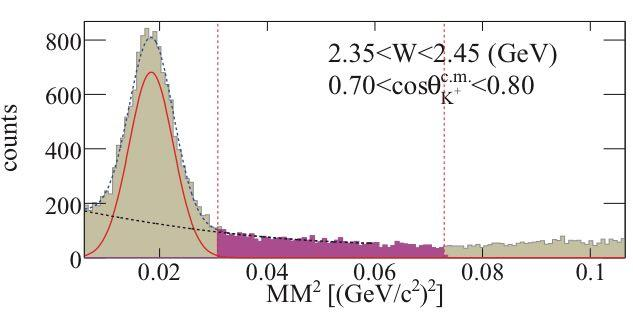
\includegraphics[width=.5\linewidth]{mism}
	\caption*{Missing  mass of the reaction $\gamma p \to K^+p\pi^-(X)$, selection range in magenta.  \citet{lineshapes}}
\end{figure}
\end{frame}




\begin{frame}{Measurements and analysis}
	\begin{itemize}
		\item now the signal regions have been established
		\item the true lineshape of the $\Lambda(1405)$ has to be extracted from the vast of reactions $\to$ any other contributions have to be substracted
		\item strategy: use of \textsc{Monte-Carlo} fits to the data, simulating the contribution of other resonances using the PDG widths and masses
		
	\end{itemize}
\end{frame}

\begin{frame}{Measurements and analysis}
some fit results:
\begin{figure}
	\centering
	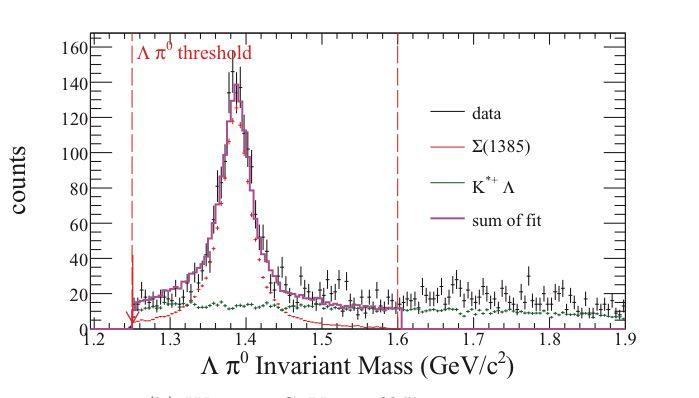
\includegraphics[width=.49\linewidth]{inv_mass_res1}
	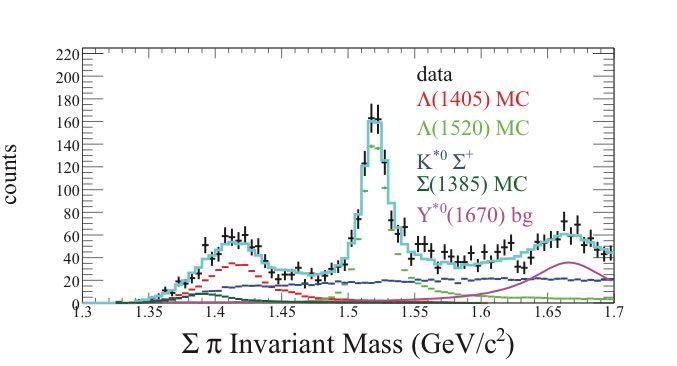
\includegraphics[width=.49\linewidth]{inv_mass_res2}
	\caption*{ Sample fit results of invariant mass spectra for a single bin in energy and angle,  \citet{lineshapes}}
	
\end{figure}
\end{frame}

\begin{frame}{Interpretation of the results}
	having substracted all unwanted reactions, one can obtain the true $\Lambda(1405)$ lineshapes:
	\begin{figure}
		\centering
		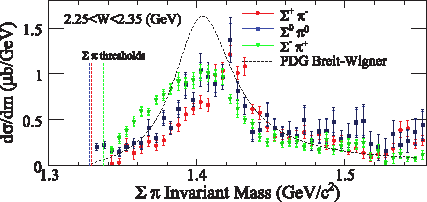
\includegraphics[width=\linewidth,angle=0]{CLAS_lineshape_compare}
		\caption*{Lineshapes of the $\Lambda(1405)$ for the 3 different decay channels and the PDG \textsc{Breit-Wigner}. The data were summed over all angles for better statistics. \citet{lineshapes}}
	\end{figure}
\end{frame}
\begin{frame}{Interpretation of the results}
 there are in fact predictions of the lineshapes differing by decay channel \citet{nacher}. \\$\to$ main idea: not one amplitude, but two due to isospin decomposition.
	\begin{figure}
		\centering
		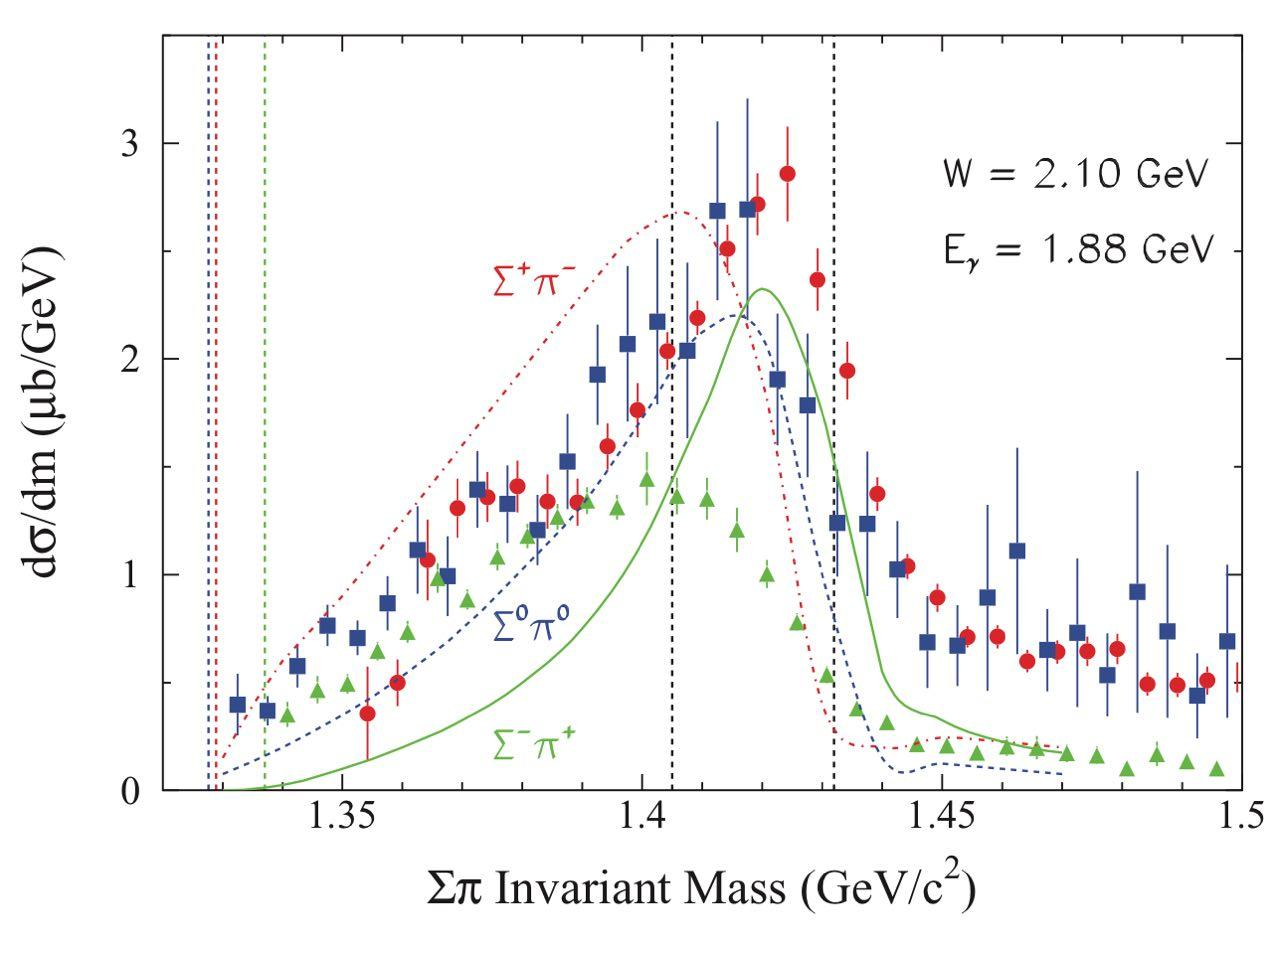
\includegraphics[width=.58\linewidth]{nacher}
		\caption*{Lineshapes of the $\Lambda(1405)$ for the 3 different decay channels and the prediction of \citet{nacher},  \citet{lineshapes}}
	\end{figure}
\end{frame}
\begin{frame}{Interpretation of the results}
	\textsc{Moriya et al.} saw two main reasons for the lineshapes differing from a simple \textsc{Breit-Wigner}:
	\begin{enumerate}
		\item isospin decomposition
		\item channel coupling between the detected $\Sigma\pi$ and $N\overline{K}$ final states
	\end{enumerate}
\begin{minipage}{.56\linewidth}
	\begin{tcolorbox}[colback=black!10,colframe=gray!20!black,title=Isospin decomposition] 
		let $$|t_I|^2=|\braket{I,0|T^{(I)}|\gamma p}|^2,$$
		then we can write (neglecting $I=2$ using CGK)
		\vspace{-0.5cm}
		\begin{align*}
			|T_{\pi^-\Sigma^+}|^2&=\frac{1}{3}|t_0|^2+\frac{1}{2}|t_1|^2-\frac{2}{\sqrt{6}}t_0t_1\cos\phi_{01}\\
			|T_{\pi^0\Sigma^0}|^2&=\frac{1}{3}|t_0|^2\\
			|T_{\pi^+\Sigma^-}|^2&=\frac{1}{3}|t_0|^2+\frac{1}{2}|t_1|^2+\frac{2}{\sqrt{6}}t_0t_1\cos\phi_{01}
		\end{align*}
	\end{tcolorbox}
\end{minipage}
\begin{minipage}{.43\linewidth}
	\begin{tcolorbox}[colback=black!10,colframe=gray!20!black,title=Channel coupling]
		the $t_I$ are described by one or two \textsc{Breit-Wigner} amplitudes with mass dependent widths $\Gamma$ \\
		$\to$ modify the amplitude preserving analyticity \citet{flatte} including the $N\overline{K}$ decay channel available at threshold\\ $m_K+m_p\approx\SI{1434}{\mega\eV}$

	\end{tcolorbox}
\end{minipage}

\end{frame}
\begin{frame}{Interpretation of results}
	fits with two $I=1$ and one $I=0$ amplitudes lead to best agreement with measured data 
	\begin{figure}
		\centering
		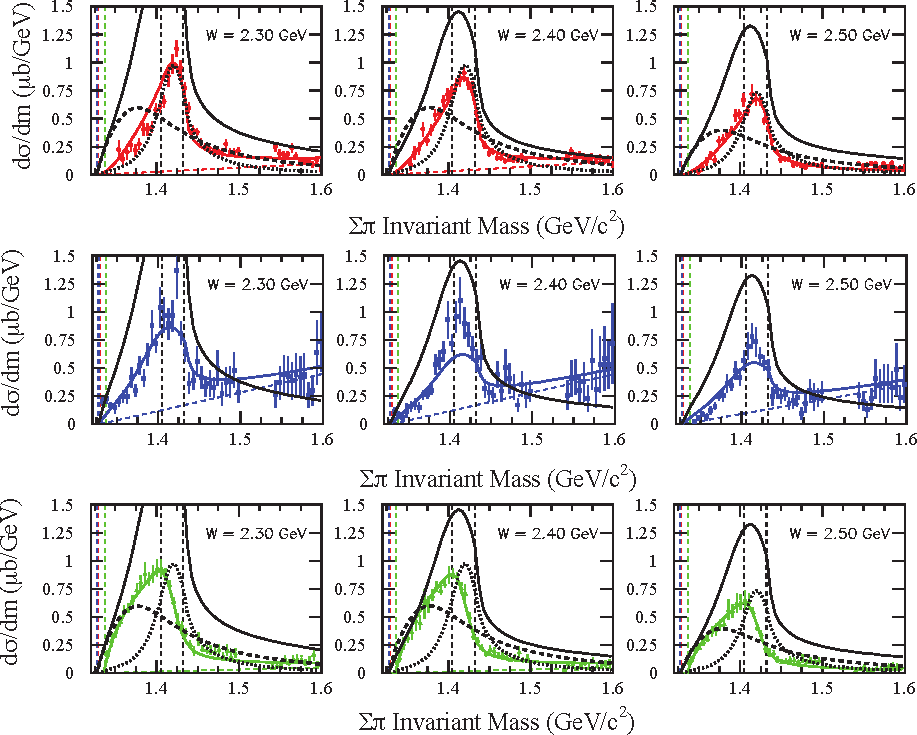
\includegraphics[width=.57\linewidth]{CLAS_lineshape_all}
		\caption*{Data and fits for $\Sigma^a\pi^b, \{a,b\}\in\{+-,00-+\}$  for different bins in $W$. $I=0$ (solid black), narrow $I=1$ (dotted black) and wide $I=1$ (dashed black). Background dashed. \citet{lineshapes}}
	\end{figure}
	
	
\end{frame}





\section{Spin-parity measurement}
\begin{frame}{Theoretical basics I}
	The $\Lambda(1405)$ is so far (mostly) assumed to have $J^P=\frac{1}{2}^-$, but this has not been determined experimentally
	\begin{tcolorbox}[colback=black!10,colframe=gray!20!black,title=Measuring spin] 
		\begin{itemize}
			\item consider the strong decay $Y^*\to Y\pi$, with $J^P$ the spin and parity of $Y^*$
			\item the $Y\pi$ angular distribution will only depend on $J$
			\begin{align*}
				I(\theta_Y)&=\text{const.} & J=1/2\\
				I(\theta_Y)&\propto 1+\frac{3(1-2p)}{2p+1}\cos^2\theta_Y& J=3/2,
			\end{align*}
			where $\theta_Y$ is the polar angle of the decay direction of $Y$ in the $Y^*$ rest frame, $p$ describes the fraction of spin projections along the $z$ axis 
			\item uniform decay pattern is best evidence for spin $J=1/2$
			
		\end{itemize}
	\end{tcolorbox}
	\begin{flushright}
		[\cite{spinparity}]
	\end{flushright}
	
\end{frame}


\begin{frame}{Measurements and analysis I }
	\begin{minipage}{\linewidth}
	\begin{tcolorbox}[colback=black!10,colframe=gray!20!black,title=Analysis procedure] 
		\begin{itemize}
			\item plot the angular distribution of the projections  $\cos\theta_\Sigma$ for each bin
			\item test each spin hypothesis using \textsc{Monte-Carlo} maximum likelihood fits, which employ angular decay probability distributions according to each hypothesis for $\Sigma\pi$ 
			\item compare each hypothesis by calculating a $\chi^2$ probability
		\end{itemize}
	\end{tcolorbox}	

\end{minipage}
\end{frame}
\begin{frame}{Meausrements and analysis I}
	\begin{figure}
		\centering
		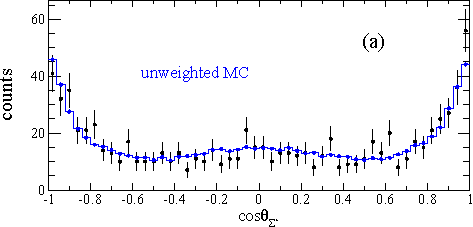
\includegraphics[width=\linewidth]{spin_half}
		\caption{Distribution of decay angle of the $\sigma^+$ with \textsc{Monte-Carlo} fit using flat templates \citet{spinparity}}
	\end{figure}
\end{frame}

\begin{frame}{Theoretical basics II}
	\begin{minipage}{.59\linewidth}
		\begin{tcolorbox}[colback=black!10,colframe=gray!20!black,title=Measuring parity] 
			\begin{itemize}
				\item the key to accessing the parity lies in determining the Polarization transfer to the decay product $Y$ which we will denote $\mathbf{Q}$
				\item the angular distribution of $\mathbf{Q}$ will only depend on $\mathbf{P}$
				\begin{align*}
				\mathbf{Q}(\theta_Y)&=\text{const.} & J^P=1/2^-\\
				\mathbf{Q}(\theta_Y)&=-\mathbf{P}+2(\mathbf{P}\cdot \mathbf{q})\mathbf{q} & J^P=1/2^+
				\end{align*}
				
				\item $\mathbf{Q}$ can be measured from weak decay angular distribution of  $Y$ 
				
			\end{itemize}
		\end{tcolorbox}		
	\end{minipage}
	\begin{minipage}{.4\linewidth}
		\begin{figure}[H]
			\centering
			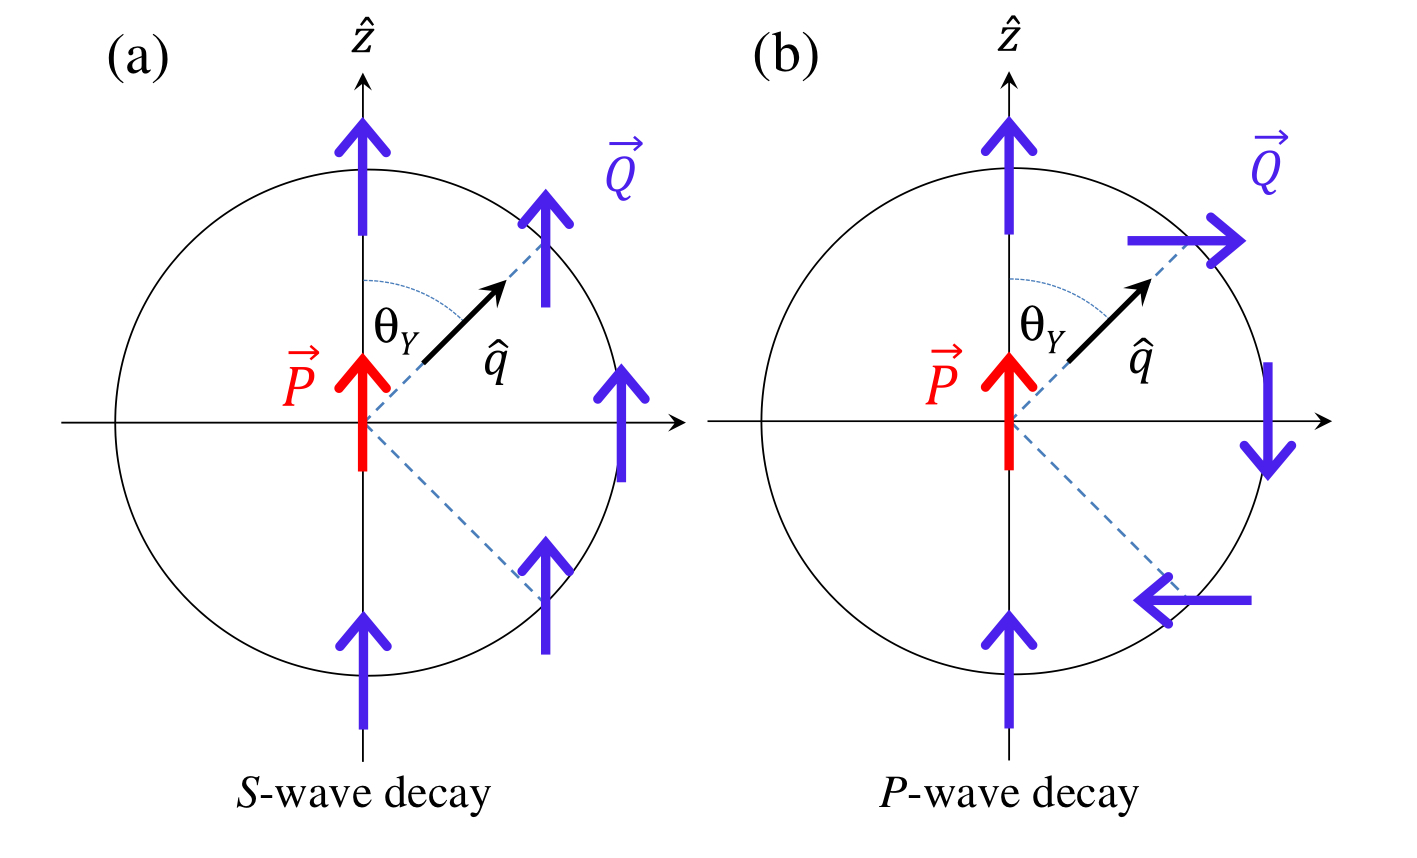
\includegraphics[width=\linewidth]{pol}
			\caption*{Polarization transfer in the strong decay $Y^*\to Y\pi$,  [\cite{spinparity}]}
		\end{figure}
	\end{minipage}
	
	\begin{flushright}
		[\cite{spinparity} and Ref. therein]
	\end{flushright}
\end{frame}

\begin{frame}{Measurements and analysis II}
		\begin{tcolorbox}[colback=black!10,colframe=gray!20!black,title=Analysis procedure] 
		\begin{itemize}
			\item plot the angular distribution of the projections  $\cos\theta_p$ for each bin
			\item determine the polarization using \textsc{Monte-Carlo} fits
			\item determine $Q_z(\cos\theta_{\Sigma^+})$ to get the parity (const. for $P=-$ quadratic for $P=+$)
		\end{itemize}
	\end{tcolorbox}	
Result: data is consistent with $J^P=1/2^-$ but does in principle not rule out $J^P=3/2^+$. $1/2^+$ and $3/2^-$ hypotheses can be discarded.
\end{frame}

\begin{frame}{Measurements and analysis II}
		\begin{figure}
			\centering
			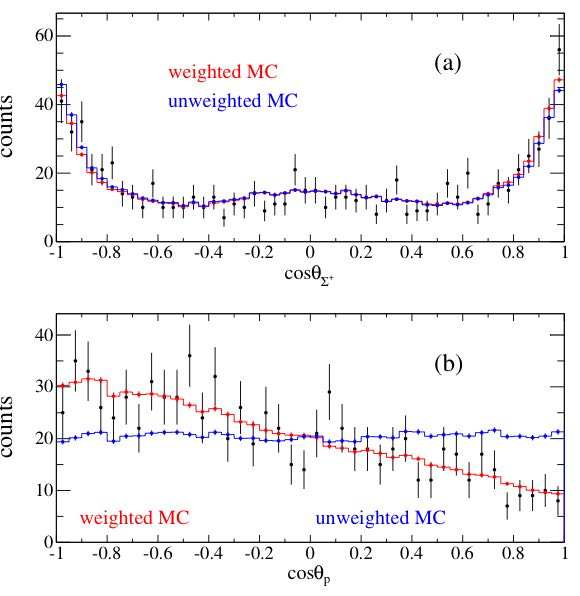
\includegraphics[width=.5\linewidth]{angular_dist}
			\caption*{Distributions of the projections of (a)$\cos\theta_\Sigma$ and (b) $\cos\theta_p$ @ $2.65<W<\SI{2.75}{\giga\eV}$ and $0.70<\cos\theta<0.80$,  \citet{spinparity}}
		\end{figure}

\end{frame}
\begin{frame}{Measurements and analysis II}
	\begin{figure}
		\centering
		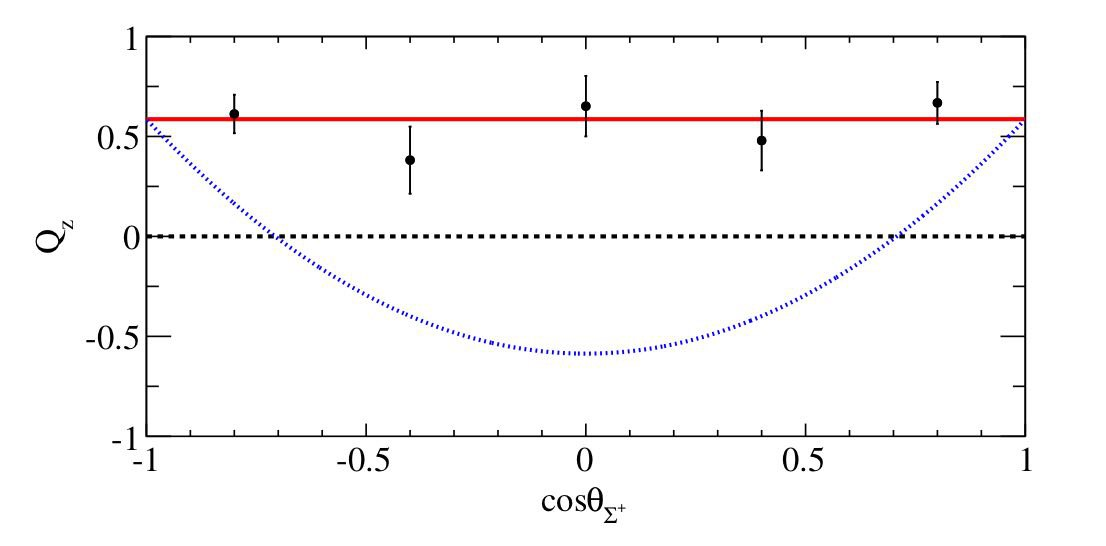
\includegraphics[width=\linewidth]{angular_pol}
		\caption*{Angular distribution of the polarization $Q_z$ @ $2.65<W<\SI{2.75}{\giga\eV}$ and $0.70<\cos\theta<0.80$. Red: average, blue: expectation for $P$-wave decay.  \citet{spinparity}}
	\end{figure}
	
\end{frame}




\section{Conclusion}
\begin{frame}{Conclusion}
\begin{minipage}{.49\linewidth}
	\begin{tcolorbox}[colback=black!10,colframe=gray!20!black,title=Lineshape measurement] 
	\begin{itemize}
		\item the CLAS detector was used to study $\gamma p \to K^+\Lambda(1405)$
		\item after selecting the correct events the true lineshape was extracted using \textsc{Monte-Carlo} sim. of the yield of other resonances
		\item the lineshapes in different decay channels differ from each other and from a simple \textsc{Breit-Wigner}
		\item a phenomenological isospin decomposition model was able to describe the data
	\end{itemize}

\end{tcolorbox}
\end{minipage}
\begin{minipage}{.49\linewidth}
	\begin{tcolorbox}[colback=black!10,colframe=gray!20!black,title=Spin parity measurement] 
		\begin{itemize}
			\item the angular distribution of the decay $\Lambda(1405)\to\Sigma^+\pi^-$ was studied
			\item the angular distributions were tested against various $J^P$ hypotheses
			\item the data is consistent with $J^P=1/2^-$ but does not exclude $J^P=3/2^+$
		\end{itemize}
		
	\end{tcolorbox}
\end{minipage}	
\end{frame}




\begin{frame}{References}
	\printbibliography
\end{frame}
\appendix
\section*{Back-Up}
\begin{frame}{Back-up: Continuous Electron Beam Accelerator Facility (CEBAF)}
	\begin{tcolorbox}[colback=black!10,colframe=gray!20!black,title=How can we access $\Lambda(1405)$ with this setup?]
		\begin{itemize}
			\item employ radiator target for the electrons
			\item generate high energy photons using the \emph{bremsstrahlung} process
			\item shoot high energy photons on proton target (LH2)
			\item then we can observe $\gamma p \to K^+\Lambda(1405)$ while knowing $p_\gamma,p_p$
		\end{itemize} 
		
	\end{tcolorbox}
\end{frame}
\begin{frame}{Back-up: Spin-Parity -- Measurements and analysis}
	\begin{minipage}{.4\linewidth}
		\begin{tcolorbox}[colback=black!10,colframe=gray!20!black,title=Event selection] 
			\begin{itemize}
				\item select kinematic region where the $\Sigma\pi$ invariant mass is dominated by the $\Lambda(1405)$ $\to M_{\Sigma\pi}\in$ \SIrange{1.30}{1.45}{\giga\eV}
				\item inspect nine bins in energy and angle, namely with CM energy at $2.6, 2.7$ and $2.8$ GeV and the  three forwardmost kaon angle bins each
			\end{itemize}
		\end{tcolorbox}	
	\end{minipage}
	\begin{minipage}{.57\linewidth}
		\begin{figure}
			\centering
			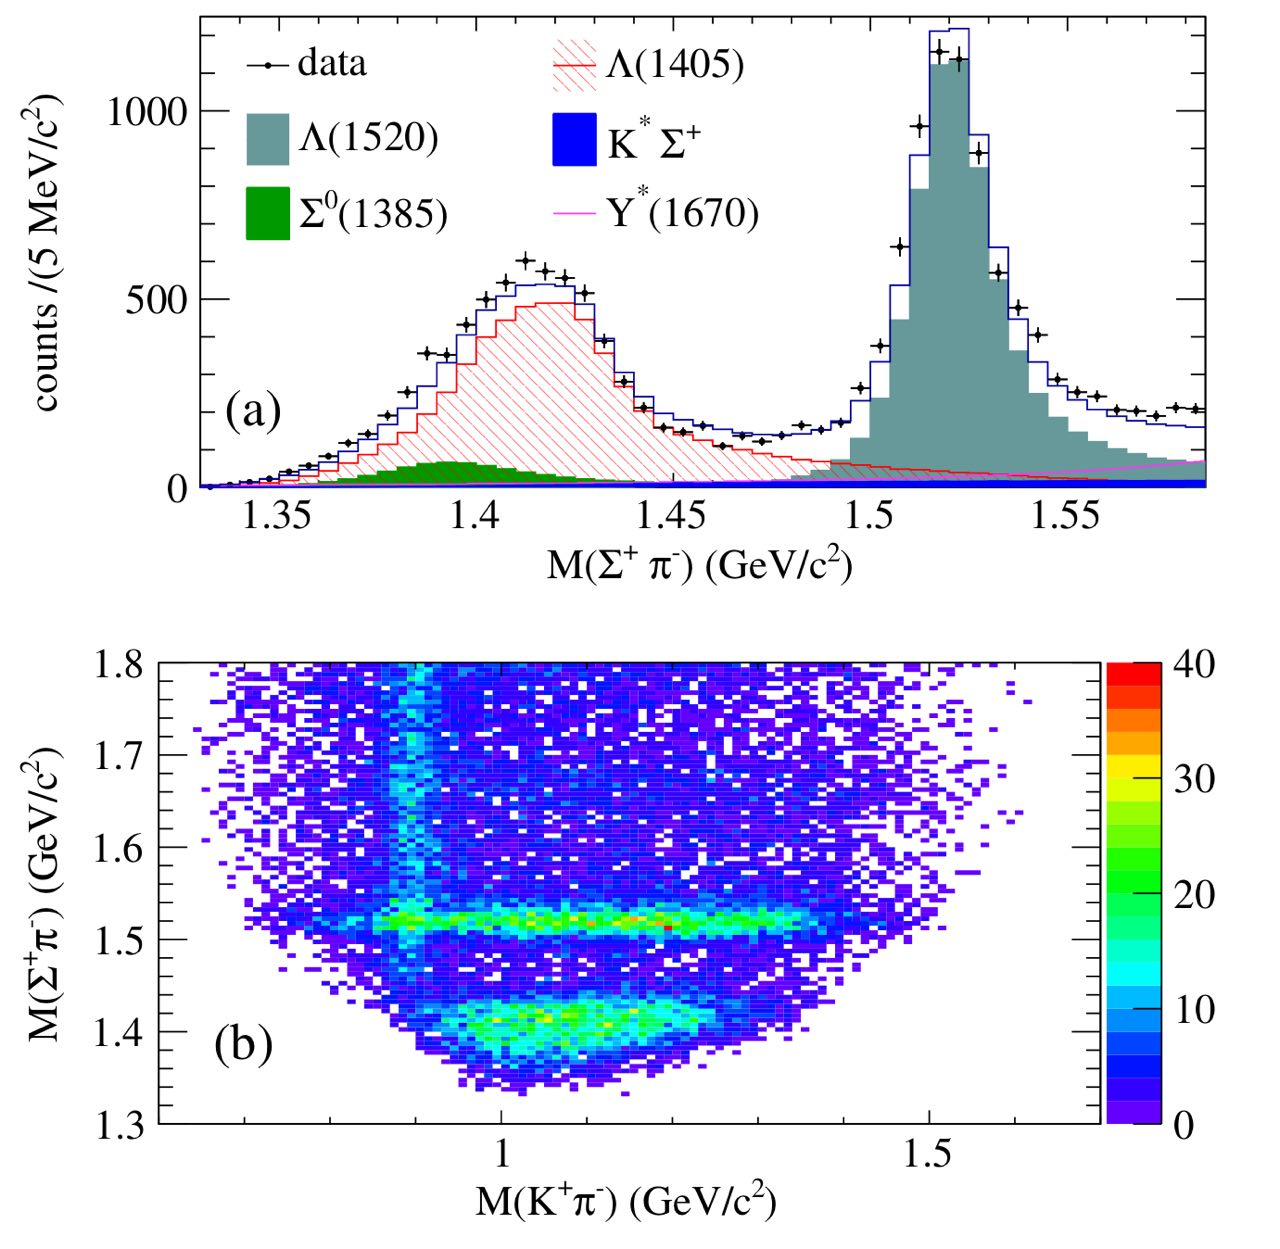
\includegraphics[width=.95\linewidth]{events_pol}
			\caption*{$\Sigma\pi$  and $K\pi$ invariant mass in the vicinity of the $\Lambda(1405)$,  [\cite{spinparity}]}
		\end{figure}
	\end{minipage}
\end{frame}

\end{document}